\subsection{RETRACTIONS AND SECTIONS}

PROPOSITION 8. Let \(f\) be a mapping of A into B. If there exists a mapping \(r\) (resp. \(s\) ) of B into A such that \(r \circ f\) (resp. \(f \circ s\) ) is the identity mapping of A (resp. B), then \(f\) is injective (resp. surjective). Conversely, if \(f\) is surjective, there exists a mapping \(s\) of B into A such that \(f \circ s\) is the identity mapping of B. If \(f\) is injective and if \(A \neq \emptyset\) , there exists a mapping \(r\) of B into A such that \(r \circ f\) is the identity mapping of A.

If there exists a mapping \(r\) of \(B\) into \(A\) such that \(r \circ f\) is the identity mapping of \(A\) , then the equality \(f(x) = f(y)\) , where \(x \in A\) and \(y \in A\) , implies \(x = r(f(x)) = r(f(y)) = y\) , and so \(f\) is injective. If there exists a mapping \(s\) of \(B\) into \(A\) such that \(f \circ s\) is the identity mapping of \(B\) , we have \(B = f(s(B)) \subset f(A) \subset B\) , so that \(f\) is surjective. If \(f\) is surjective, let \(T\) denote the term \(\tau_y(y \in A \text{ and } f(y) = x)\) . We have \(f(T) = x\) for \(x \in B\) ; if \(s\) denotes the mapping \(x \to T (x \in B, T \in A)\) , then \(f \circ s\) is the identity mapping of \(B\) . Finally, suppose that \(f\) is injective and that \(A \neq \emptyset\) , and let \(a\) be an element of \(A\) . The relation

\[
" (y \in A \text {   and   } x = f (y)) \text {   or   } (y = a \text {   and   } x \in B - f (A))"
\]

implies \((x, y) \in \mathbf{B} \times \mathbf{A}\) and therefore has a graph \(\mathbf{R}\) with respect to the letters \(x, y\) . This graph is functional by reason of the hypothesis on \(f\) , and has \(\mathbf{B}\) as its domain; and we have \(\mathbf{R}(x) = a\) if \(x \in \mathbf{B} - f(\mathbf{A})\) , and \(f(\mathbf{R}(x)) = x\) if \(x \in f(\mathbf{A})\) . Hence the function \(r = (\mathbf{R}, \mathbf{B}, \mathbf{A})\) is such that \(r \circ f\) is the identity mapping of \(\mathbf{A}\) .

COROLLARY. Let A, B be sets, let f be a mapping of A into B, and let g be a mapping of B into A. If \(g \circ f\) is the identity mapping of A and if \(f \circ g\) is the identity mapping of B, then f and g are bijective, and \(g = \overline{f}^{1}\) .

DEFINITION 11. Let \(f\) be an injective (resp. surjective) mapping of A into B. Any mapping \(r\) (resp. s) of B into A such that \(r \circ f\) (resp. \(f \circ s\) ) is the identity mapping of A (resp. B) is called a retraction (resp. section) of \(f\) .

Instead of retraction (resp. section) the phrase left-inverse (resp. right-inverse) is sometimes used.

If \(f\) is injective (resp. surjective) and if \(r\) (resp. \(s\) ) is a retraction (resp. section) of \(f\) , then \(f\) is a section (resp. retraction) of \(r\) (resp. \(s\) ). Hence a retraction is surjective and a section is injective.

If \(f\) is surjective and if \(s, s'\) are two sections of \(f\) such that \(s(\mathbf{B}) = s'(\mathbf{B})\) , then \(s = s'\) ; for if \(x \in \mathbf{B}\) , there exists \(y \in \mathbf{B}\) such that \(s(x) = s'(y)\) , and we have \(x = f(s(x)) = f(s'(y)) = y\) , so that \(s(x) = s'(x)\) and consequently \(s = s'\) . Thus a section \(s\) is uniquely determined by the set \(s(\mathbf{B})\) . By abuse of language, the set \(s(\mathbf{B})\) is sometimes called a section of \(f\) .

THEOREM 1. Let \(f\) be a mapping of A into B, let \(f'\) be a mapping of B into C, and let \(f'' = f' \circ f\) . Then :

\begin{enumerate}
\def\labelenumi{(\alph{enumi})}
\item
  If \(f\) and \(f'\) are injections, then \(f''\) is an injection. If \(r, r'\) are retractions of \(f, f'\) , respectively, then \(r \circ r'\) is a retraction of \(f''\) .
\item
  If \(f\) and \(f'\) are surjections, then \(f''\) is a surjection. If \(s, s'\) are sections of \(f, f'\) , respectively, then \(s \circ s'\) is a section of \(f''\) .
\item
  If \(f''\) is an injection, then \(f\) is an injection. If \(r''\) is a retraction of \(f''\) , then \(r'' \circ f'\) is a retraction of \(f\) .
\item
  If \(f''\) is a surjection, then \(f'\) is a surjection. If \(s''\) is a section of \(f''\) , then \(f \circ s''\) is a section of \(f'\) .
\item
  If \(f''\) is a surjection and \(f'\) an injection, then \(f\) is a surjection. If \(s''\) is a section of \(f''\) , then \(s'' \circ f'\) is a section of \(f\) .
\item
  If \(f''\) is an injection and \(f\) a surjection, then \(f'\) is an injection. If \(r''\) is a retraction of \(f''\) , then \(f \circ r''\) is a retraction of \(f'\) .
\end{enumerate}

For every set E let \(I_{E}\) denote the identity mapping of E.

\begin{enumerate}
\def\labelenumi{(\alph{enumi})}
\tightlist
\item
  We have \(r \circ f = I_A\) and \(r' \circ f' = I_B\) , hence
\end{enumerate}

\[
\left(r \circ r ^ {\prime}\right) \circ \left(f ^ {\prime} \circ f\right) = r \circ I _ {B} \circ f = r \circ f = I _ {A}.
\]

If \(f\) and \(f'\) are injections, then \(f''\) is an injection, by Proposition 8 if \(A \neq \emptyset\) , and trivially if \(A = \emptyset\) .

\begin{enumerate}
\def\labelenumi{(\alph{enumi})}
\setcounter{enumi}{1}
\tightlist
\item
  We have \(f \circ s = \mathbf{I}_{\mathrm{B}}\) and \(f' \circ s' = \mathbf{I}_{\mathrm{C}}\) , hence
\end{enumerate}

\[
(f ^ {\prime} \circ f) (s \circ s ^ {\prime}) = f ^ {\prime} \circ I _ {B} \circ s ^ {\prime} = f ^ {\prime} \circ s ^ {\prime} = I _ {C}.
\]

If \(f\) and \(f'\) are surjections, \(f''\) is then a surjection by Proposition 8.

\begin{enumerate}
\def\labelenumi{(\alph{enumi})}
\setcounter{enumi}{2}
\item
  We have \(r'' \circ f'' = I_A\) , hence \((r'' \circ f') \circ f = r'' \circ f'' = I_A\) . If \(f''\) is an injection, then \(f\) is an injection, by Proposition 8 if \(A \neq \emptyset\) , and trivially if \(A = \emptyset\) .
\item
  We have \(f'' \circ s'' = I_C\) , hence \(f' \circ (f \circ s'') = f'' \circ s'' = I_C\) . If \(f''\) is a surjection, then \(f'\) is a surjection by Proposition 8.
\item
  We have \(f'' \circ s'' = I_G\) , and \(f'\) is a bijection by (d). Hence
\end{enumerate}

\[
\begin{array}{r l} f \circ (s ^ {\prime \prime} \circ f ^ {\prime}) = (\bar {f} ^ {1 ^ {\prime}} \circ f ^ {\prime}) \circ f \circ (s ^ {\prime \prime} \circ f ^ {\prime}) & = \bar {f} ^ {1 ^ {\prime}} \circ (f ^ {\prime \prime} \circ s ^ {\prime \prime}) \circ f ^ {\prime} \\ & = \bar {f} ^ {1 ^ {\prime}} \circ I _ {C} \circ f ^ {\prime} = \bar {f} ^ {1 ^ {\prime}} \circ f ^ {\prime} = I _ {B}. \end{array}
\]

If \(f''\) is a surjection and \(f'\) an injection, \(f\) is then a surjection by Proposition 8.

\begin{enumerate}
\def\labelenumi{(\alph{enumi})}
\setcounter{enumi}{5}
\tightlist
\item
  We have \(r'' \circ f'' = I_A\) , and \(f\) is a bijection by (c). Hence
\end{enumerate}

\[
\begin{array}{r l} \left(f \circ r ^ {\prime \prime}\right) \circ f ^ {\prime} = \left(f \circ r ^ {\prime \prime}\right) \circ f ^ {\prime} \circ \left(f \circ \overline {{f}} ^ {1}\right) & = f \circ \left(r ^ {\prime \prime} \circ f ^ {\prime \prime}\right) \circ \overline {{f}} ^ {1} = f \circ I _ {A} \circ \overline {{f}} ^ {1} \\ & = f \circ \overline {{f}} ^ {1} = I _ {B}. \end{array}
\]

If \(f''\) is an injection and \(f\) a surjection, then \(f'\) is an injection, by Proposition 8 if \(A \neq \emptyset\) , and trivially if \(A = \emptyset\) (for then we have \(B = f\langle A\rangle = \emptyset\) ).

PROPOSITION 9. (a) Let E, F, G be sets, let g be a mapping of E onto F and f a mapping of E into G. Then there exists a mapping h of F into G such that \(f = h \circ g\) if and only if the relation \(g(x) = g(y)\) (where \(x \in E\) , \(y \in E\) ) implies the relation \(f(x) = f(y)\) . The mapping h is then uniquely determined by f; if s is a section of g, we have \(h = f \circ s\) .

\pandocbounded{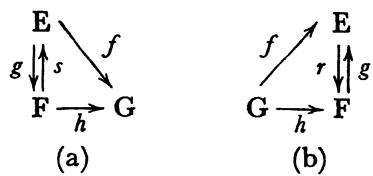
\includegraphics[keepaspectratio]{images/part001_ef8e01c05a3dcb28772fb1963be4c012627d42ff76089463ce60c193ac31650a.jpg}}

\begin{enumerate}
\def\labelenumi{(\alph{enumi})}
\setcounter{enumi}{1}
\item
  Let E, F, G be sets, let g be an injection of F into E, and let f be a mapping of G into E. Then there exists a mapping h of G into F such that \(f = g \circ h\) if and only if \(f(\mathbf{G}) \subset f(\mathbf{F})\) . The mapping h is uniquely determined by f; if r is a retraction of g, we have \(h = r \circ f\) .
\item
  If \(f = h \circ g\) , the relation \(g(x) = g(y)\) (where \(x \in \mathbf{E}\) , \(y \in \mathbf{E}\) ) clearly implies \(f(x) = f(y)\) . And for every section \(s\) of \(g\) we have
\end{enumerate}

\[
h = h \circ (g \circ s) = f \circ s,
\]

which shows that h is uniquely determined by f.~Conversely, suppose that the relation \(g(x) = g(y)\) implies \(f(x) = f(y)\) ; let s be a section of \(g\) , and let \(h = f \circ s\) ; then for every \(x \in \mathbf{E}\) we have \(g(s(g(x))) = g(x)\) , hence \(f(s(g(x))) = f(x)\) , that is, \(h(g(x)) = f(x)\) and therefore \(f = h \circ g\) .

\begin{enumerate}
\def\labelenumi{(\alph{enumi})}
\setcounter{enumi}{1}
\tightlist
\item
  If \(f = g \circ h\) , then clearly \(f(\mathbf{G}) \subset f(\mathbf{F})\) , and for every retraction \(r\) of \(g\) we have \(h = (r \circ g) \circ h = r \circ f\) , which shows that \(h\) is uniquely determined by \(f\) . Conversely, suppose that \(f(\mathbf{G}) \subset f(\mathbf{F})\) ; let \(r\) be a retraction of \(g\) , and put \(h = r \circ f\) ; for every \(x \in \mathbf{G}\) , there exists \(y \in \mathbf{F}\) such that \(f(x) = g(y)\) , so that
\end{enumerate}

\[
g (h (x)) = g (r (f (x))) = g (r (g (y))) = g (y) = f (x)
\]

and therefore \(f = g \circ h\) .

